\section{Reducing the Number of Calculations}\label{sec:barnes}
\subsection{The problem}
As we have seen in the introduction, Newton's equation \eqref{Newton G} applies on every object in our solar system.
\begin{equation}
\frac{d^2\vec{r}_i}{dt^2}=G\sum_{j\neq i}m_j\frac{\vec{r_j}-\vec{r_i}}{|\vec{r_j}-\vec{r_i}|^3}
\label{Newton G}
\end{equation}
 Thus, for every of the $N$ objects in the system, the pairwise forces of the other $N-1$ objects need be calculated. This means that for every time step $\Delta t$, the number of calculations equals $N(N-1)$. Therefore the brute force algorithm has complexity $\orde{N^2}$. For 1000 objects and 12000 time steps, one need to perform at most $1000^2\cdot 12000 = 12000000000$ (12 billion) calculations -- collisions excluded. This results in an extremely slow program on most computers.
\subsection{The Barnes-Hut algorithm: a partial solution}
To reduce the amount of calculations on equation \eqref{Newton G}, we make use of the \textit{Barnes-Hut Algorithm} \cite{barneshut}. The general idea is to treat objects that are 'sufficiently near each other' in comparison to their distance from the considered object, as one.\\
\\
\textbf{Algorithm}
\begin{enumerate}
\item Choose a parameter $\theta \in \R_{>0}$.
\item Create a tree, called the Barnes-Hut tree, whose root contains the center of mass and total mass of all objects. Next, choose a length $L$, such that the hypercube with length $L$ and center the center of mass, encapsulates all objects. For speed, $L$ is usually chosen as small as possible.
\item If this hypercube contains only one object (or no objects), we do nothing; otherwise, cut the hypercube in half in every dimension, and for every such created subspace, create a child of the root that represents that subspace, including the total mass and center of mass of the objects in that subspace.\label{cutinhalf}
\item For every such created subspace, recursively repeat step \ref{cutinhalf} until every subspace has zero or one object.
\item For every object $a$, do the following.
\begin{enumerate}
\item Start at the root of the Barnes-Hut tree.
\item For the current node, if the node represents zero objects, do nothing. If the node represents one object, calculate the force that object excerts on $a$. If the node represents more than one object, and thus is an internal node, calculate the ratio $\frac{s}{d}$, where $s$ is the length of the space - that is, the distance between a corner point and a closest other corner point - represented by the node, and $d$ is the distance between the center of mass of the node and $a$.\label{calculate}
\item If the node is internal and $\frac{s}{d}<\theta$, then treat the node as a single object with mass and center of mass of that node. Otherwise, recursively repeat \ref{calculate} and \ref{treatsingle} for the node's children.\label{treatsingle}
\end{enumerate}
\end{enumerate}
\newpage
\textbf{Example.} Consider the following map, which is a more detailed example than in \cite{barneshut}.
\begin{figure}[H]
\centering
\begin{subfigure}{0.35\textwidth}
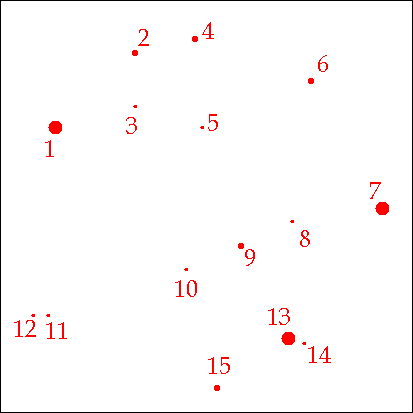
\includegraphics[width=\textwidth]{barneshut_map.png}
\caption{An example of a map with objects. The boundary of the map is already given.}
\end{subfigure}\hspace{1cm}
\begin{subfigure}{0.35\textwidth}
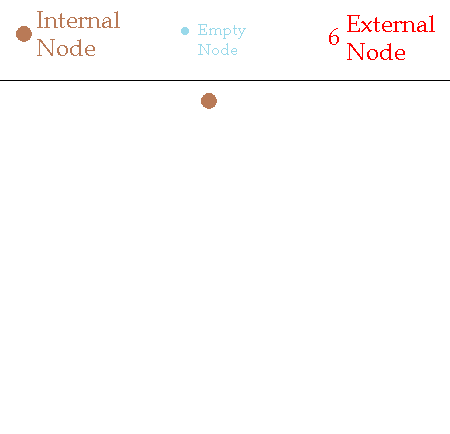
\includegraphics[width=\textwidth]{barneshut_tree_root.png}
\caption{The current tree, containing only the root.}
\end{subfigure}
\caption{The starting situation}
\end{figure}
Splitting the space and filling the tree, we get the following result.
\begin{figure}[H]
\centering
\begin{subfigure}{0.35\textwidth}
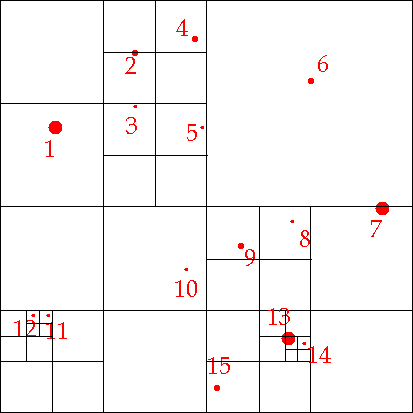
\includegraphics[width=\textwidth]{barneshut_map_devided.png}
\caption{An example of a map with objects. Now the space is divided in subspaces such that every object has its own subspace.}
\end{subfigure}\hspace{1cm}
\begin{subfigure}{0.35\textwidth}
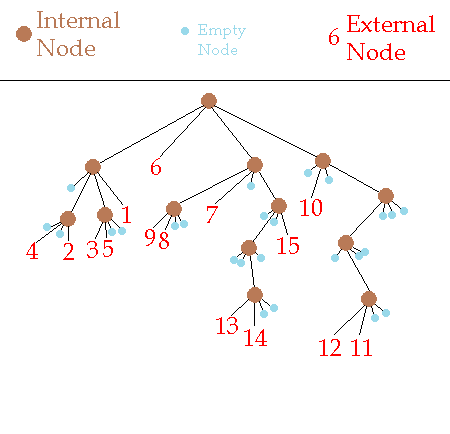
\includegraphics[width=\textwidth]{barneshut_tree.png}
\caption{The final tree}
\end{subfigure}
\caption{The final situation}
\end{figure}
Note that we build the tree, starting from the northwest subspace of a node and proceeding clockwise.\\

Assume that we want to calculate the net force on object 15, with $\theta = \frac{1}{3}$ as the chosen parameter. In this case, both the root and its children do not satisfy $\frac{s}{d} < \frac{1}{3}$, since 6 is an external node, we add the pairwise force between 6 and 15 to 15's net force. Moving one level down, any node with center of mass outside the green zone showed below can be treated as one object. The \textit{level} of a node is the number of ancestors the node has. In example: the root has level 0, its children level 1.
\begin{figure}[H]
\centering
\begin{subfigure}{0.24\textwidth}
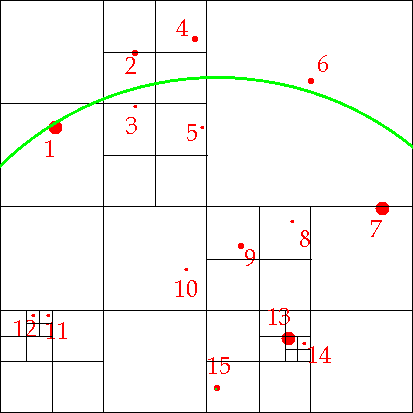
\includegraphics[width=\textwidth]{barneshut_map_green_2.png}
\caption{The green zone indicates which internal nodes can be treated as one (outside), and which can't (inside).}
\end{subfigure}\hspace{1cm}
\begin{subfigure}{0.24\textwidth}
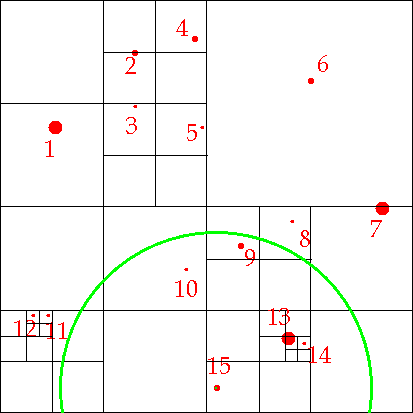
\includegraphics[width=\textwidth]{barneshut_map_green_3.png}
\caption{The green zone indicates which internal nodes can be treated as one (outside), and which can't (inside).}
\end{subfigure}\hspace{1cm}
\begin{subfigure}{0.24\textwidth}
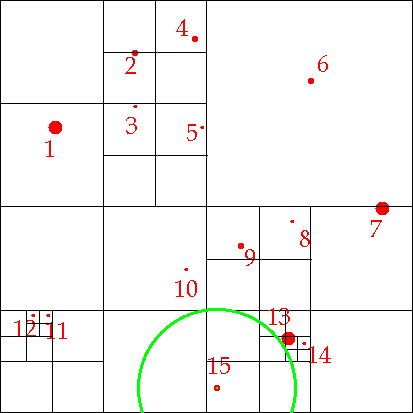
\includegraphics[width=\textwidth]{barneshut_map_green_4.png}
\caption{The green zone indicates which internal nodes can be treated as one (outside), and which can't (inside).}
\end{subfigure}\hspace{1cm}
\begin{subfigure}{0.24\textwidth}
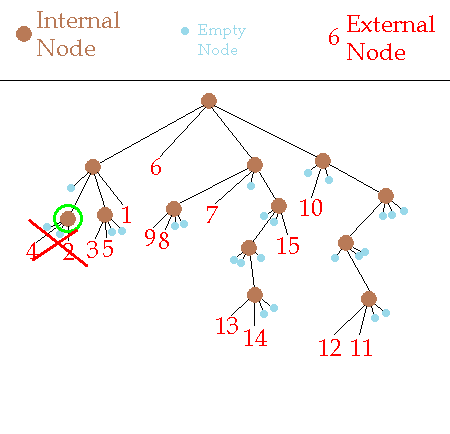
\includegraphics[width=\textwidth]{barneshut_tree_node_4_2.png}
\caption{The green node can be treated as a single object.}
\end{subfigure}\hspace{1cm}
\begin{subfigure}{0.24\textwidth}
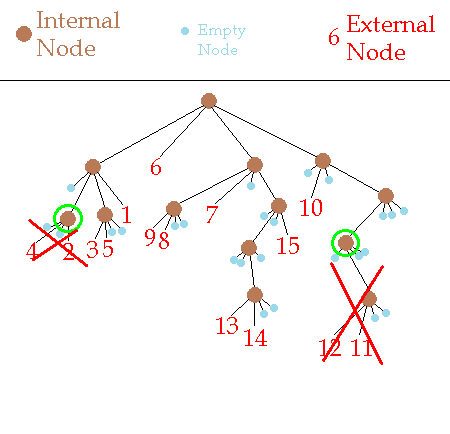
\includegraphics[width=\textwidth]{barneshut_tree_node_lvl3.png}
\caption{The green node can be treated as a single object.}
\end{subfigure}\hspace{1cm}
\begin{subfigure}{0.24\textwidth}
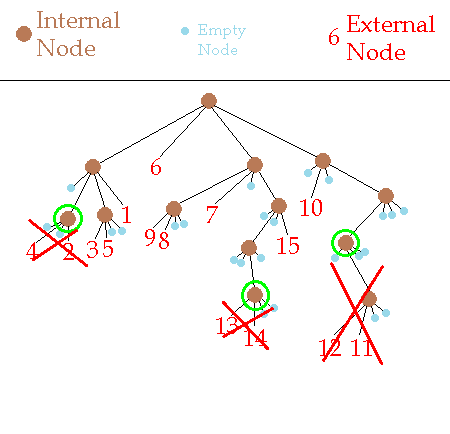
\includegraphics[width=\textwidth]{barneshut_tree_node_lvl4.png}
\caption{The green node can be treated as a single object.}
\end{subfigure}
\caption{Check which nodes can be treated as one object, at different levels (root is level 0, root's children are level 1, etc.): left corresponds to level 2, center to level 3, right to level 4.}\label{fig:check}
\end{figure}
Figure \ref{fig:check} indicates that we must calculate the pairwise forces of object 15 with objects 1, 3, 5, 6, 7, 8, 9, 10, but we can group objects 2 and 4, 11 and 12, and 13 and 14 to be treated as one object to calculate the force on object 15.
The computer uses the algorithm recursively, so it will first check the first child of the root, its children, etc, before moving on to the root's second child.

\subsection{Analysis: complexity}
The strength of the Barnes-Hut algorithm is that the tree is built only once per time step. Thus, for every object one just has to 'walk through the tree' without having to create it. We will make this point more specific.
\subsubsection*{Building the tree} Using the same terminology as in the previous example, we can note that, for every level of the tree, there are at most $N$ objects represented by the nodes of that level. For a node representing $k$ objects, calculating the center of mass takes $2k$ elementary operations ($k$ multiplications and $k$ additions), and the calculation of the total mass takes $k$ additions. So in total there are $3k$ elementary operations. Therefore, for every level, there are at most $3N$ elementary operations to do.\\
Now looking at the number of levels, we can give a lower bound but unfortunately no upper bound. For a $D$-dimensional space, a node has ideally $2^D$ children with an equal amount of objects. In this case there will be $\ceiling{^{2^D} \log(N)} = \ceiling{\frac{^2\log(N)}{D}}$ levels, which is the lower bound.\\
Unfortunately, there can't be said anything about the upper bound; simply take one object to be randomly far away from two others. In this case, the tree just goes down and every node contains exactly the same information as it's parent, except for the last one, which has two external children. Fortunately, according to our simulations, the vast majority of the time, the number of levels isn't much greater than the lower bound. Assuming the lower bound, we have a complexity for building the tree of $\orde{N\log(N)}$.
\subsubsection*{Number of calculations, given a tree} Let $i$ be a given object, and $D$ the dimension of our space. As we have seen in the example, we can draw a hypersphere, with center the location $\vec{r}_i$ of $i$, outside which a node can be treated as a single object. Since this hypersphere changes in size according to the size of the piece of space represented by the node, there's a constant maximum $M_\theta$ of nodes of a certain level that fall \textit{inside} the sphere corresponding to the same level. If for that particular level holds
\[
2^D M_\theta \leq 2^{D\cdot \text{level}}
\]
the other $M_\theta(2^D-1)$ fall outside and can be calculated. For the remaining levels, this amount is even less. Thus, for every level the number of calculations is at most
\[
M_\theta (2^D-1) := c(\theta)
\]
so the number of calculations for every level is bounded by a constant.\\

We have noted earlier that there is no upper bound for the number of levels. However, with the number of levels approximately $\orde{\log(N)}$, the total number of calculations for object $i$ should be $\orde{\log(N)}$. Therefore the total number of calculations on one time step is $\orde{N\log(N)}$, but again this is on average, not worst case.
\subsection{Analysis: Precision and the Size of the Error}
As one can expect, the precision of the Barnes-Hut algorithm is solely dependent on its only parameter $\theta$. We will first make a few remarks.
\begin{enumerate}
\item Let $D$ be the dimension of the considered space, and suppose $\theta > \frac{1}{\sqrt{D}}$. Consider the condition $\frac{s}{d} < \theta$. This implies
\[
s < d\theta > \frac{d}{\sqrt{D}}
\]
Thus, $s$ might be greater than $\frac{d}{\sqrt{D}}$. Suppose this is the case. Noting that the distance between two objects in the same subspace is at most $\sqrt{Ds^2} = s\sqrt{D}$, this implies $s\geq d$. So, the algorithm considers an object in the same subspace as to be sufficient far away. In this case the algorithm lets an object excert force on itself -- strictly forbidden. So $\theta \leq \frac{1}{\sqrt{D}}$ must hold. We will see later that strictly less applies.
\item Note that the calculated force is always less than or equal to the actual force if the objects are aligned with respect to the object $a$ on which the force is calculated. If the objects are next to each other with respect to $a$ and have the same distance to $a$, however, the calculated force is greater due to the "head-tail" method. Usually, the calculated force is less than the actual force.
Thus, $s$ might be greater than $\frac{d}{\sqrt{D}}$. Noting that the distance between two objects in the same subspace is at most $\sqrt{Ds^2} = s\sqrt{D}$, which might imply $s\geq d$. So, it might be that the algorithm considers an object in the same subspace as to be sufficient far away. In this case the algorithm lets an object excert force on itself -- strictly forbidden. So $\theta$ must be smaller than $\frac{1}{\sqrt{D}}$. We will see later that strictly smaller applies.

\item Note that the calculated force is always less than or equal to the actual force, if the objects are aligned with respect to the object $a$ on which the force is calculated on. If the objects are next to each other with respect to $a$ and have the same distance to $a$, however, the calculated force is greater due to the "head-tail" method. Usually, the calculated force is less than the actual force.
\item Consider a subspace represented by a node, that contains two objects. Let $d_1$ be the distance from the considered object to the first object, and let $d_2$ be defined similarly. In addition, let $m_1$ be the mass of the first object and $m_2$ the mass of the second object. Consider the error in the force calculated
\[
E(m_1,m_2,d_1,d_2) = \frac{m_1}{d_1^2}+\frac{m_2}{d_2^2}-\frac{m}{d^2}
\]
where $m = m_1+m_2$ and $d = \frac{m_1d_1+m_2d_2}{m}$ is the center of mass.\\
We will prove that the error reaches no maximum in terms of $\Delta d$. Suppose
\[
\begin{array}{cc}
m_2 = cm_1, c\in \R_{>0}, & d_2-d_1 = \Delta d
\end{array}
\]
We can now express $m_1,m_2,d_1,d_2$ in terms of $m,d,c,\Delta d$: one can easily check that
\begin{align*}
m_1 &= \frac{1}{1+c}m\\
m_2 &= \frac{c}{1+c}m\\
d_1 &= d-\frac{m_2}{m}\Delta d = d-\frac{c}{1+c}\Delta d\\
d_2 &= d+\frac{m_1}{m}\Delta d = d+\frac{1}{1+c}\Delta d
\end{align*}
Now the error reduces to
\[
E = \frac{m\frac{1}{1+c}}{(d-\frac{c}{1+c}\Delta d)^2}+\frac{m\frac{c}{1+c}}{(d+\frac{1}{1+c}\Delta d)^2}-\frac{m}{d^2}
\]
To determine the extrema of this error with respect to $\Delta d$, we take the derivative to $\Delta d$.
\begin{align*}
\frac{\partial E}{\partial \Delta d} &= \frac{m}{1+c}\left(d-\frac{c}{1+c}\Delta d\right)^{-3}2\frac{c}{1+c}+\frac{mc}{1+c}\left(d+\frac{1}{1+c}\Delta d\right)^{-3}\left(-2\frac{1}{1+c}\right)\\
&= 2\frac{mc}{(1+c)^2}\left(\left(d-\frac{c}{1+c}\Delta d\right)^{-3}-\left(d+\frac{1}{1+c}\Delta d\right)^{-3}\right)
\end{align*}
Setting this derivative equal to zero reduces to
\[
\left(d-\frac{c}{1+c}\Delta d\right)^3 = \left(d+\frac{1}{1+c}\Delta d\right)^3
\]
which is equivalent to
\[
\Delta d\left(\Delta d^2\frac{1+c^3}{(1+c)^3}+3d\Delta d\frac{1-c^2}{(1+c)^2}+3d^2\right) = 0
\]
Without loss of generality, we can state $d=1$, since $d$ is expressed in some unit, and $\Delta d$ is expressed in the same unit. This leads to
\begin{equation}
\Delta d = 0, \text{ or } \frac{1+c^3}{(1+c)^3}\Delta d^2+3\frac{1-c^2}{(1+c)^2}\Delta d+3 = 0
\end{equation}
The discriminant of the second equation equals
\begin{equation}
\frac{(1-c^2)^2}{(1+c)^4}-12\frac{1+c^3}{(1+c)^3} = \frac{(1-c)^2}{(1+c)^2}-12\left(1-\frac{3c}{(1+c)^2}\right) = \frac{c^2+34c+1}{(1+c)^2}-12 = \frac{32c}{(1+c)^2}-11
\end{equation}
Setting the discriminant to zero yields another equation
\begin{equation}
11c^2-10c+11 = 0
\end{equation}
of which the discriminant is strictly less than zero, which implies no solution $c\in \R$.\\
Thus, $\Delta d=0$ is the only solution, which implies that the error is smallest when $\Delta d=0$, which may be expected, but also that there is no other extremum, which proves there is no maximum in the error in terms of $\Delta d$.\hfill $\qedsymbol$
\item For simplicity, we can always take the situation as described above, since two objects in the same subspace can be exactly grouped into one at a place inside the subspace. So, we can assume a node contains two objects, for our error analysis. Furthermore, for simplicity, we only look at the error in the \textit{magnitude}, not the direction, since they are related by the shape of our subspaces.

\end{enumerate}

We can now start our error analysis.
As in remark (3), assume there are two objects in the considered subspace, and let $m_1,m_2,d_1,d_2,m,d,c,\Delta d$ as in remark (3), and, without loss of generality, assume $m = d = 1$. By remark (3) we can assume $\Delta d$ has its maximum value, which equals
\[
\Delta d = s\sqrt{D} < d\theta \sqrt{D} = \theta\sqrt{D}
\]
and the error reduces to
\[
E = \frac{1}{(1+c)(1-\frac{c}{1+c}\Delta d)^2}+\frac{c}{(1+c)(1+\frac{1}{1+c}\Delta d)^2}-1
\]
Since we are interested in the supremum of the error, we can take the limit $\Delta d \rightarrow \theta \sqrt{D}$. By remark (1), we may assume $\theta < \sqrt{D}$, and therefore $\Delta d<1$.\\
Since $\Delta d$ is now fixed, we can take the derivative of the error to the ratio of mass $c$ in order to determine the supremum of the error given any parameter $\theta$. Instead, we use MATLABs \textit{patternsearch} function. The result for $D=2$ is given in Table \ref{tab:maxerror}.
\begin{table}[h!]
\centering
\caption{The maximum value of the error for various values of $\theta$. The last column includes the ratio of masses for the worst case scenario to occur.}
\label{tab:maxerror}
\begin{tabular}{c|c|c}
$\theta$ & Maximum Value of the Error & $c$\\
\hline
$\frac{1}{\sqrt{2}}$ & $\infty$ & $\infty$\\
$1/2$ & $0.6782$ & $3.4431$\\
$2/5$ & $0.334$ & $2.4064$\\
$1/3$ & $0.2068$ & $2.0022$\\
$1/4$ & $0.1052$ & $1.6439$\\
$1/5$ & $0.0645$ & $1.4767$\\
$1/6$ & $0.0438$ & $1.3792$\\
$1/8$ & $0.0241$ & $1.2696$\\
$1/12$ & $0.0105$ & $1.1712$\\
$1/16$ & $0.0059$ & $1.1255$ 
\end{tabular}
\end{table}\\
\textbf{Remark.} Despite the theoretically large error, choosing $\theta = \frac{1}{2}$ or even larger usually suffices, as long as $\theta < \frac{1}{\sqrt{2}}$. There are two reasons for this. First, the actual error is much smaller most of the time. Second, the objects on the other side reduce the error. Put more precisely, by remark (2), errors in the calculations of forces exerted by objects on either side of the considered object are subtracted from each other, reducing the total error.
\subsection{Using the Barnes Hut Tree to Reduce the Number of Collision Tests}
In the initial model, for every celestial body $i$, we test whether a collision takes place for every celestial body $j>i$. The Barnes Hut tree can be used to reduce the number collision tests in the model. Therefore, for every body $i$, we set a rectangle around the object bounded by it's minimum and maximum position according to the linearized path function $\gamma_i$ (see section 'The Model' for precise details), as follows.
\[
\begin{array}{ll}
\textbf{if } \vec{v}_{i,1} >= 0 &\\
& x_{max,i} = \vec{x}_{i,1}+r_i+\vec{v}_{i,1}\Delta t\\
& x_{min,i} = \vec{x}_{i,1}-r_i\\
\textbf{else }\\
& x_{max,i} = \vec{x}_{i,1}+r_i\\
& x_{min,i} = \vec{x}_{i,1}-r_i+\vec{v}_{i,1}\Delta t\\
\textbf{if } \vec{v}_{i,2} >= 0 & \\
& y_{max,i} = \vec{x}_{i,2}+r_i+\vec{v}_{i,2}\Delta t\\
& y_{min,i} = \vec{x}_{i,2}-r_i\\
\textbf{else } & \\
& y_{max,i} = \vec{x}_{i,2}+r_i\\
& y_{min,i} = \vec{x}_{i,2}-r_i+\vec{v}_{i,2}\Delta t\\
\end{array}
\]
For internal nodes of the tree, we take $x_{max}$ to be the maximum of the $x_{max,i}$ of the objects represented by the node. $x_{min},y_{max},y_{min}$ are defined similarly. Figure \ref{fig:grenzen} illustrates this principle.
\begin{figure}[H]
  \centering
  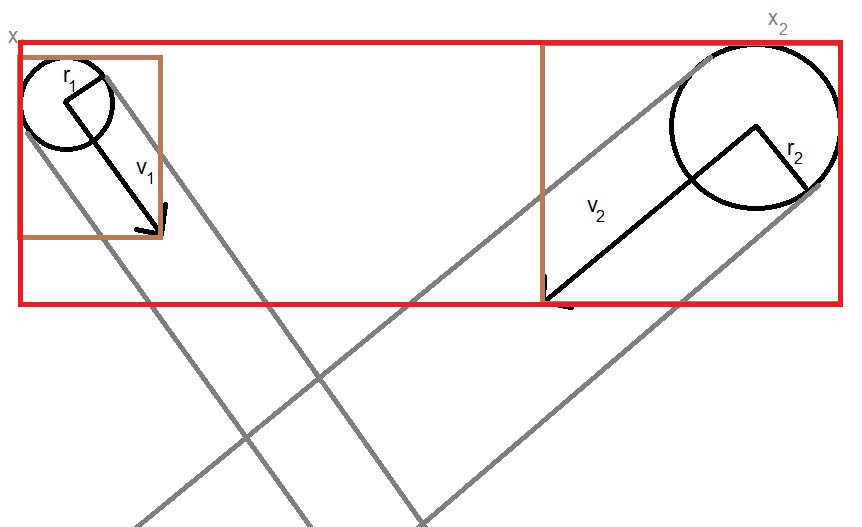
\includegraphics[width=0.5\textwidth]{boundaries}
  \caption{An illustration of two celestial bodies, with the above defined boundaries for the individual bodies (brown) and the node representing the two bodies (red).}
  \label{fig:grenzen}
\end{figure}
Similar to the Barnes Hut algorithm with forces, the collision algorithm recursively checks whether the boundaries of the current considered object and the current node overlap; if so, check it's children, if not, move on. After this process a list of bodies is set on which a collision test is performed. Similarly, one can easily check that the number of collision tests reduces to $\orde{N\log(N)}$ when this algorithm is used.\\
\textbf{Remark.} Note that, in contrast to the force algorithm, the collision algorithm is an exact algorithm -- without loss of precision. That is, it produces the same result as the brute force algorithm. Thus, the collision algorithm doesn't need an extra parameter.
\subsection{Conclusion and Implementation}
Reducing the number of calculations on Newton's equation can be done with the Barnes Hut algorithm, but not without loss of precision. However, even using a parameter such as $\theta=\frac{1}{2}$ practically suffices for most uses. We chose to use $\theta = \frac{1}{2}$ in our simulations. Since the Barnes Hut tree is built only once per time step, the number of calculations reduces from $\orde{N^2}$ to $\orde{N\log(N)}$.\\
Furthermore, a variation on the Barnes Hut algorithm can be used to reduce the number of collision tests on any object. This goes without loss of precision and also has order of complexity $\orde{N\log N}$. We implemented this algorithm in our model as well.\\
However, even with these improvements on the speed, simulating still takes a long time with the use of personal computers.

